\documentclass[answers]{exam}

% ------------------------------------------------------------------------------ %
% -----------------------      Base for every .tex file   ---------------------- %
% ------------------------------------------------------------------------------ %

\usepackage[dvipsnames]{xcolor}
\usepackage{mathtools}
\usepackage{amssymb}
\usepackage{amsthm}
\usepackage{amsmath}
\usepackage{framed}
\usepackage{wasysym}
\usepackage{geometry}
\usepackage{cancel}
\usepackage{blindtext}
\usepackage{pgfplots}
\usepackage{graphicx}
\usepackage{lastpage}
\usepackage[most]{tcolorbox} 
\usepackage{multicol}
\usepackage{soul}
\usepackage{listings}
\usepackage{algorithm}
\usepackage{algorithmic}
\usepackage{booktabs}
\usepackage{tikz}
\usepackage{pifont}

% Libraries
\usetikzlibrary{shapes,shapes.geometric, positioning, arrows}

\geometry{%
	left=15mm,
	right=15mm,
	top=25mm,
	bottom=25mm,
	bindingoffset=0mm,
	headheight=30pt,% output from geometry tells you what this needs to be set to as a minimum
}

% Header and Footer
\pagestyle{headandfoot}
\firstpageheadrule
\runningheadrule
\firstpageheader{Convex Optimization}{\today}{Jonathan Schnell}
\runningheader{Convex Optimization}{}{Jonathan Schnell}
\firstpagefooter{}{Page \thepage\ of \numpages}{}
\runningfooter{}{Page \thepage\ of \numpages}{}

% Commands
\newcommand{\imp}[1]{\ul{\textbf{#1}}}
\newcommand{\dproduct}[1]{\left\langle #1 \right\rangle}
\newcommand{\norm}[1]{\left\lVert #1 \right\rVert}
\renewcommand{\vector}[1]{\begin{pmatrix} #1 \end{pmatrix}}
\newcommand{\abs}[1]{\left| #1 \right|}
\newcommand{\floor}[1]{\lfloor #1 \rfloor}
\newcommand{\ceil}[1]{\lceil #1 \rceil}
\newcommand{\fracpart}[2]{\frac{\partial #1}{\partial #2}}
\newcommand{\set}[2]{\left\{#1 \ \middle|\ #2\right\}}
\renewcommand{\hat}[1]{\widehat{#1}}

\newcommand{\Ker}{\operatorname{Ker}}
\renewcommand{\Im}{\operatorname{Im}}
\renewcommand{\Re}{\operatorname{Re}}
\renewcommand{\dim}{\operatorname{dim}}
\renewcommand{\div}{\operatorname{div}}
\newcommand{\rot}{\operatorname{rot}}
\newcommand{\grad}{\operatorname{grad}}
\newcommand{\vol}{\operatorname{vol}}
\newcommand{\supp}{\operatorname{supp}}
\renewcommand{\div}{\operatorname{div}}
\newcommand*{\vertbar}{\rule[-1ex]{0.5pt}{2.5ex}}
\newcommand*{\horzbar}{\rule[.5ex]{2.5ex}{0.5pt}}

\theoremstyle{definition}
\newtheorem*{definition}{Definition}
\newtheorem*{beispiel}{Beispiel}
\newtheorem*{remark}{Remark}

\theoremstyle{plain}
\newtheorem*{proposition}{Proposition}
\newtheorem*{satz}{Satz}
\newtheorem*{korollar}{Korollar}
\newtheorem*{lemma}{Lemma}
\newtheorem*{theorem}{Theorem}


% Quote
\newtcolorbox{zitat}[1]{%
	colback=lightGray,
	grow to right by=-10mm,
	grow to left by=-10mm, 
	boxrule=0pt,
	boxsep=0pt,
	breakable,
	enhanced jigsaw,
	borderline west={4pt}{0pt}{gray},
	#1
}

% Use colors in equations
\newcommand{\highlight}[2]{\colorbox{#1}{$#2$}}%
\definecolor{lightGray}{gray}{0.9} 

% To add shortcut of script Letters in Equations
\newcommand{\s}[1]{\mathcal{#1}}
\newcommand*\circled[1]{\tikz[baseline=(char.base)]{
            \node[shape=circle,draw,inner sep=2pt] (char) {#1};}}
\newcommand{\cmark}{\ding{51}}
\newcommand{\xmark}{\ding{55}}


\newenvironment{claim}[1]{
		\par\noindent
		\textbf{Claim.} #1
		\begin{tcolorbox}[blanker, top=3mm, bottom=3mm, left=3mm, borderline west={1pt}{0mm}{black}]
		\noindent\textit{Proof of Claim.} 
}{
	\hfill$\blacksquare$	
	\end{tcolorbox}\noindent
}

% To add shortcut of number's set Z
\newcommand*{\Z}{\mathbb{Z}}
\newcommand*{\N}{\mathbb{N}}
\newcommand*{\R}{\mathbb{R}}
\newcommand*{\Q}{\mathbb{Q}}
\newcommand*{\C}{\mathbb{C}}
\newcommand*{\F}{\mathbb{F}}
\newcommand*{\K}{\mathbb{K}}

% To add shortcut of empty set
\renewcommand*{\o}{\varnothing}
\pgfplotsset{compat=1.9}

\everymath{\displaystyle}

% Line-Height
\linespread{1.15}

\graphicspath{{Files/}}

% ------------------------------

\begin{document}

	$ $
	\begin{center}
		\huge \textbf{Exercise session notes - Week 2}  \\ \vspace*{3mm}
        \Large{Conic optimization programs}
	\end{center}
	$ $\\
    
	Today we introduced the conic optimization program, as an example of the convex optimization program (Chapter 2.2 in the course notes). Recall that a cone is a set $K\subseteq \R^n$ such that  
	$$ x\in K,\ \lambda\in \R_{\geq 0}\implies \lambda\cdot x \in K $$ 
	Moreover a cone is said to be proper, if it is solid ($\operatorname*{int}(K)\neq \o$), pointed (it contains no lines), convex and closed.
	\begin{definition}
		Let $K\subseteq \R^n$ be a proper cone and let $A\in \R^{m\times n}$, $b\in \R^m$ and $c\in \R^n$. A \imp{conic program} has the following form:
		\begin{alignat*}{3}
			\min\quad c^{\top} x& && \leftarrow \text{affine objective}\\ 
			Ax &= b &&\leftarrow \text{linear constraint}\\ 
			x&\in K\quad\quad &&\leftarrow \text{$x$ in the cone}
		\end{alignat*}
	\end{definition}	
	So for the following example, the feasible set of the optimization program is the orange set.
	\begin{center}
		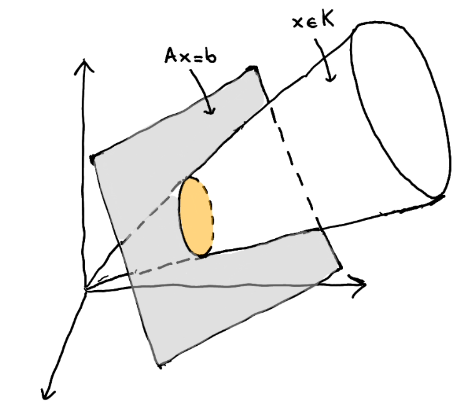
\includegraphics[width=0.4\textwidth]{ExampleConicProgram.PNG}
	\end{center}
	For a conic optimization program we can also define its dual formulation.
	\begin{definition}
		Let $K\subseteq \R^n$ be a proper cone and let $A\in \R^{m\times n}$, $b\in \R^m$ and $c\in \R^n$. The \imp{dual formulation} of a conic optimization program in standard form is	
		\begin{align*}
			\max\quad\quad b^{\top} y&\\ 
			c- A^\top y &\in K^*
		\end{align*}
		where $K^*$ is the dual cone of $K$, i.e.
		$$ K^* = \set{y\in \R^n}{y^\top x \geq 0\quad\forall x\in K} $$
	\end{definition}
	These formulation can be also extended to a general vector space instead of $\R^n$, for example the set of polynomials with real coefficients.
	\begin{remark}
		As we saw in the lecture, if we pick $K = \R^n_{\geq 0}$ the non negative orthant (recall that $\R^n_{\geq 0}$ is a proper cone and self dual), then we will get the primal-dual formulation of LPs:
		\begin{align*}
			\text{Primal:} \quad\quad\quad&& \text{Dual:}\quad\quad\quad\quad\quad&\\
			\min\quad c^{\top} x&& \max \quad\quad b^\top y &\\ 
			Ax &= b & c-A^\top y &\in \R_{\geq 0}^n\\
			x &\in \R^n_{\geq 0} & &
		\end{align*}
	\end{remark}
	An important theorem about conic optimization programs is the weak duality theorem. It says that the optimal value of the dual always gives us a lower bound on the optimal value of the primal.
	\begin{theorem}[Weak duality for conic programs]
		Let $x,y$ be feasible solutions to the primal-dual formulation of some conic program. Then 
		$$ c^\top x \geq b^\top y $$
	\end{theorem}
	\begin{proof}
		Let $x,y$ feasible solutions, then 
		\begin{align*}
			c^\top x -y^\top b &= c^\top x - y^\top Ax &\text{($Ax = b$)}\\ 
			&= c^\top x - (A^\top y)^\top x &\\ 
			&= (c - A^\top y)^\top x&\\ 
			&\geq 0 & \text{($c - A^\top y\in K^*$)}
		\end{align*}
	\end{proof}
	For linear programs there is also a theorem called Strong Duality, which says that the gap between the primal optimal value and the dual optimal value is zero. Unfortunately, this theorem holds unconditionally only for LPs. Later in the course we will see an example of conic program for which strong duality does not hold, and give sufficient conditions under which strong duality does hold.



\end{document}